\documentclass[11,aspectratio=1610]{beamer}
\usepackage[utf8]{inputenc}
\usepackage{mathrsfs}  
\usepackage{xcolor}
\usepackage{setspace}
\usepackage{comment}
\usepackage{hyperref}
% config du thgeme metropolis
\usetheme[progressbar=frametitle,block=fill, titleformat=smallcaps,sectionpage=progressbar,]{metropolis}



\title{Resilience and stability of ecological systems}
\subtitle{une article de recherche de C.S. Holling, paru en 1973}
\date{}
\author{}



\definecolor{links}{HTML}{60bbf7}
\hypersetup{colorlinks,linkcolor=,urlcolor=links}


%definition de la couleur du texte dans la balise \alert{}
\definecolor{vertIGN}{HTML}{96C31E} % vert IGN %vrai valeur #97BE0D
\setbeamercolor{alerted text}{fg=vertIGN}

\definecolor{grisIGN}{HTML}{22292F} % Gris IGN tiré vers le noir 
\setbeamercolor{background canvas}{bg=grisIGN}




% code pour placer le log ENSG dans le bandeau des slides titre 
\makeatletter
\setbeamertemplate{frametitle}{%
  \nointerlineskip%
  \begin{beamercolorbox}[%
      wd=\paperwidth,%
      sep=0pt,%
      leftskip=\metropolis@frametitle@padding,%
      rightskip=\metropolis@frametitle@padding,%
    ]{frametitle}%
  \metropolis@frametitlestrut@start%
  \insertframetitle%
  \nolinebreak%
  \metropolis@frametitlestrut@end%
  \hfill
  \raisebox{-0.6ex}{
\includegraphics[height=2.5ex,keepaspectratio]{img/logo_LASTIG.png}}
  \end{beamercolorbox}%
}
\makeatother




% logo ENSG première page 
\titlegraphic{\flushright
\includegraphics[height=1cm]{img/logo_LASTIG.png}

\vspace{7cm}
\centering

%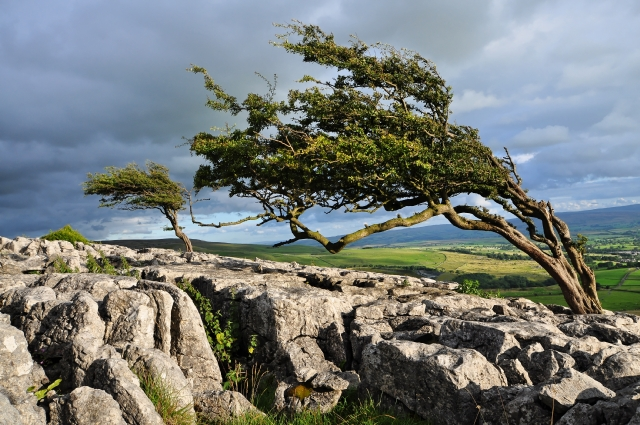
\includegraphics[height=4cm]{img/resilient_tree.jpg}\\

\begin{scriptsize}LASTIG  - 27 juin 2024 - Paul Chapron\end{scriptsize}
} 



\begin{document}
\metroset{background=dark} % change background theme according to manual
\maketitle  




\begin{frame}{Mise en garde}

Dans cette présentation
\begin{itemize}
  \item pas d'IA
  \item pas de SIG
  \item pas de cartes
  \item pas de sujets de recherche du LASTIG 
  \item pas d'expertise
\end{itemize}

\end{frame}


\section{L'auteur} 

\begin{frame}{C.S. Holling, la légende}



 \begin{columns}
          \column{0.38\textwidth}
             \centering
             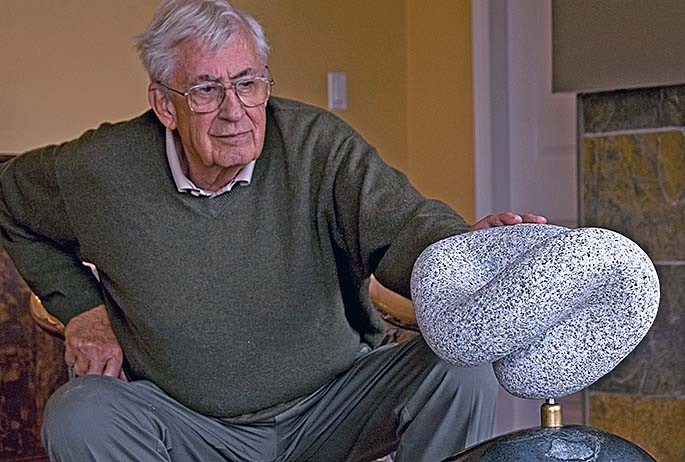
\includegraphics[width=\textwidth]{img/Holling.jpg}
           \column{0.58\linewidth}
\begin{scriptsize}
Crawford Stanley "Buzz" Holling, (1930 - 2019)

\begin{itemize}
  \item thèse d'écologie en 1957
  \item travaille plusieurs années au département Forestier du Canada (Canadian Forestry Departement )
  \item Professeur et Directeur du Institute of Animal Resource Ecology, Univ. of British Columbia 
  \item Nombreux titres et récompenses pour son travail 
\end{itemize}
\end{scriptsize}
\end{columns}

\begin{small}
\vspace{1cm}
Père du concept de \alert{résilience} +   adaptive management, adaptive cycle, and panarchy. 

\vspace{0.5 cm}
Pionnier dans les ateliers de modélisation participatifs et \alert{interdisciplinaires} de \alert{gestion de ressources naturelles}. 




\end{small}

\end{frame}


\section{La modélisation d'écosystèmes en trois diapos}




\begin{frame}{(1) Silver Springs model  }
Flux d'énergie dans les systèmes naturels  [Odum,  1971]
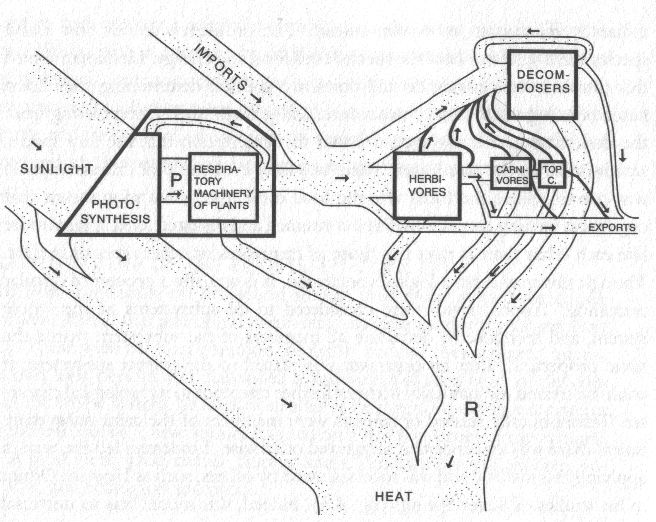
\includegraphics[width=0.8\textwidth]{img/Silver_Spring_Model.jpeg} 

\tiny{image  : via wikipedia from:  Odum, H.T. (1971). Environment, Power, and Society. Wiley-Interscience New York, N.Y.}
\end{frame}



\begin{frame}{(2) Réponses fonctionnelles}
\begin{scriptsize}

 \begin{columns}
          \column{0.38\textwidth}
             \centering
             \colorbox{white}{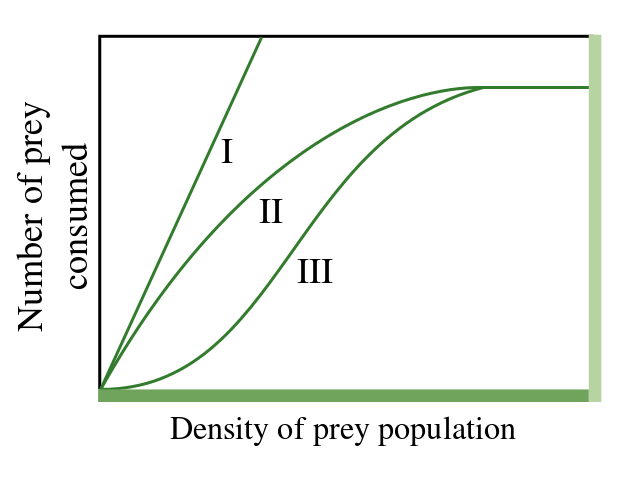
\includegraphics[width=\textwidth]{img/FunctionalResponses.png}}
           \column{0.58\linewidth}

\begin{itemize}
  \item premier travaux de Holling ~ 
  \item modélise l'influence entre la densité de rpoies et la prédations 
  \item Type I : modèle simpliste, prédation instantanée, pas de seuils ni de limites (e.g. baleine)  
  \item Type II : saturation, plateau de prédation (chasse courte, et satiété rapide) )
  \item Type III : plus rare , adaptation et choix de la proie , apprentissage
\end{itemize}
\end{columns}

\vspace{1cm}

$\rightarrow$ prédateurs se nourrissent souvent de plusieurs proies , combinant Type II et  Type III 
\end{scriptsize}
\end{frame}


\begin{frame}{(3) Modèles d'Écosystemes  }


\begin{columns}
          \column{0.7\textwidth}
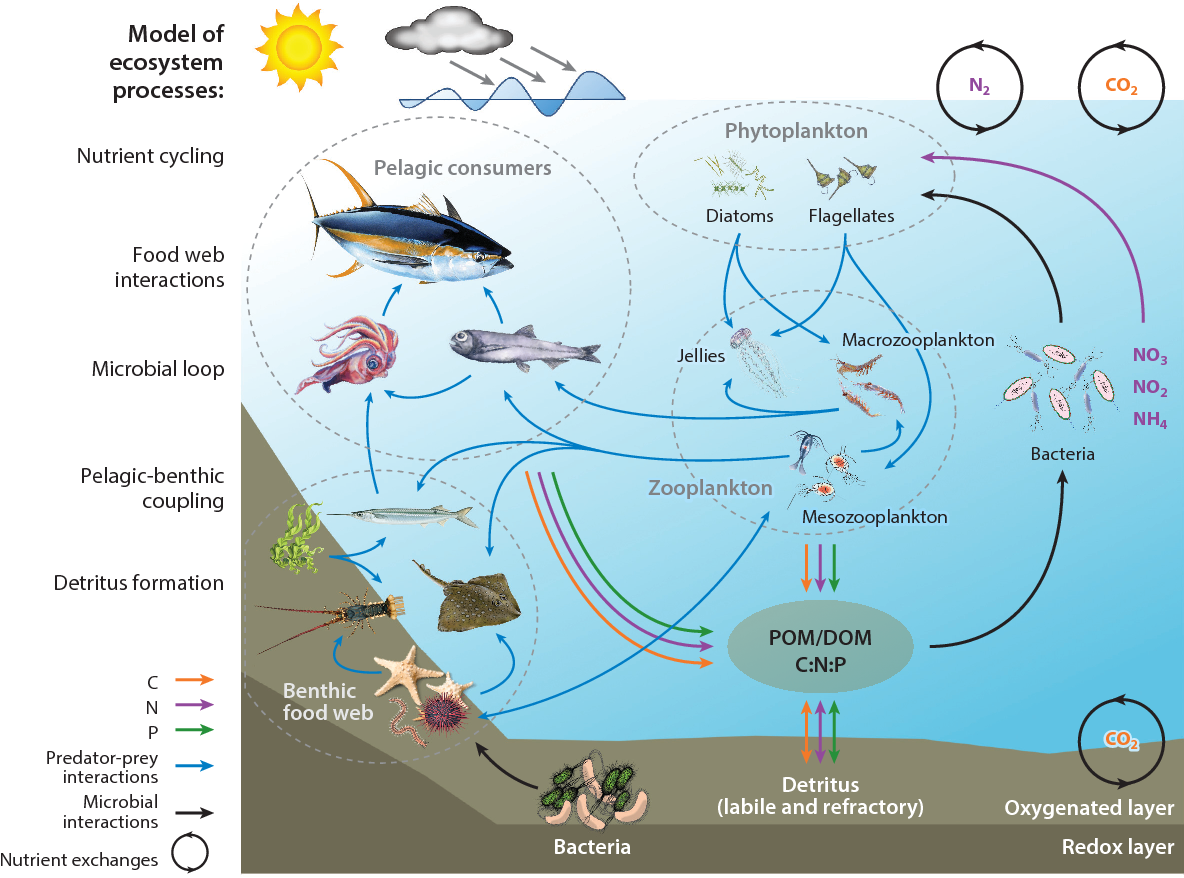
\includegraphics[width=0.9\textwidth]{img/ecosystem_model.png}
\column{0.4\textwidth}
\scriptsize{
Un  \alert{modèle d'écosystème } représente les interactions de plusieurs espèces, entre elles et avec l'environnement.


\vspace{0.5cm}
  \alert{Chaque flèche }  doit être modélisée  e.g. Réponses fonctionnelles entre le thon et ses proies 
}
\end{columns}



\vfill
\tiny{Image from :  Pethybridge, Heidi R. et al. “Improving Marine Ecosystem Models with Biochemical Tracers.” Annual review of marine science 10 (2018): 199-228.}

\end{frame}





\section{L'article}

\begin{frame}[standout]

\begin{quote}
"Individuals die, population disappear and species become extinct. That is one view of the world."
\end{quote}
\flushright
\tiny{(the first two lines of the paper)}
  
\end{frame}




\begin{frame}{Two perspectives on system}

Holling distingue deux  perspectives : 

\vspace{1cm}

\begin{scriptsize}
\begin{columns}
          \begin{column}{0.5\textwidth}
\begin{itemize}
\item quand un système est conçu pour fonctionner \alert{dans une gamme de conditions extérieures} connues et de faible magnitude  (e.g. frigo) 
\item \alert{la performance moyenne } et  connaître l'amplitude et la fréquence des oscillations est important
\item Questions \alert{quantitatives}: Combien ? Combien de plus ? Combien de temps ? 
\end{itemize}      
\end{column}
\vrule
\begin{column}{0.5\textwidth}
\begin{itemize}
\item quand un système est sensible, profondément affecté par des perturbations (e.g. grenouilles dans une mare)
\item confronté à des  \alert{variations inattendues} , un comportement consistant est \alert{moins important}  que la persistance de ses propriétés et des relations du système avec le reste du monde
\item Questions \alert{qualitatives} : Est-ce que ça existe ?  Est-ce que ça va disparaître ?  Revenir ? 
\end{itemize}
\end{column}
\end{columns}
\end{scriptsize}

\end{frame}




\begin{frame}{Tradition Quantitative}


Tradition de l'analyse  \alert{quantitative} des choses : e.g. physique,  

  \vfill

\begin{itemize}
  \item   Les équilibres sont "statiques"   (mais il existe des équilibres dynamiques: le )
  \item  Les comportements \alert{transitoires}  (i.e. loin de l'équilibre) sont mal connus 
  \end{itemize}
  \vfill
  Des limitations : 
  \begin{itemize}
  \item  Connaître l'état des populations dans des états d'équilibre  ne nous dit rien sur les conditions  de persistance
  \item  L'exploitation humaine des systèmes naturels les \alert{éloigne}  de leur positions d'équilibre
\end{itemize}
\end{frame}
  
  

\begin{frame}{Le but de l'article }
Holling fait \alert{une revue d'écologie théorique} mixée avec des  comportements observés dans de \alert{vrais écosystèmes naturels} \\ 

\vfill

$\implies$ Changer de perspective va peut-être révéler des propriétés intéressantes ?  

\vfill
Les systèmes naturels sont \alert{dynamiques}, sujet à des \alert{perturbations} (très souvent d'origine humaine). \\

\vfill
\alert{Persistance, résistance, adaptation} sont les propriétés qui nous intéressent ici






\end{frame}
  

\section{Proies et prédateurs }





\begin{frame}{Modéliser des proies et des prédateurs  }



les $\color{cyan}{proies}$ , et les $\color{orange}{predateurs}$ 


\vfill

"Les proies mangent ce qu'ils trouvent dans l'environnement"\\
"Plus il y a de prédateurs , moins il y a de proies"\\
"Plus il y a de proies plus elles peuvent se reproduire"

\vfill

"Plus les prédateurs mangent , plus ils se reproduisent"\\
"Si les prédateurs n'ont rien à manger ils meurent"

\vfill


\[
\left\{
 \begin{array}{ccc}  
 dyna \textcolor{cyan}{(proies)}&=&  +  \textcolor{cyan}{manger} +  \textcolor{cyan}{reproduire} - \textcolor{orange}{chasse}\textcolor{cyan}{(proies)}\\
 \\
dyna\textcolor{orange}{(predat)}&=&  +  \textcolor{orange}{reproduire} + \textcolor{orange}{manger}\textcolor{cyan}{(proies)} - \textcolor{orange}{famine}  \end{array}
\right.
\]

  

\end{frame}




\begin{frame}{équations de Lotka Volterra }


Modèle théorique de deux populations qui évolutent dans le temps ($t$)

$\color{cyan}{x(t)}$ les proies , $\color{orange}{y(t)}$ les prédateurs .


\[
\left\{
 \begin{array}{ccc}  
 \frac{\mathrm{d}\textcolor{cyan}{x(t)}}{\mathrm{d}t}&=&  \alpha \textcolor{cyan}{x(t)} - \beta \textcolor{cyan}{x(t)}\textcolor{orange}{y(t)}\\
 \\
\frac{\mathrm{d}\textcolor{orange}{y(t)}}{\mathrm{d}t}&=&  \delta \textcolor{cyan}{x(t)}\textcolor{orange}{y(t)} - \gamma \textcolor{orange}{y(t)}  \end{array}
\right.
\]

  

with : 
\begin{footnotesize}
\begin{itemize}
  \item  $\alpha >0$ natalité des proies 
  \item  $\beta >0 $ mort des proies par prédation
  \item  $\gamma >0 $ mortalité des prédateurs
  \item  $\delta > 0$  reproductions des prédateurs quand ils prédatent
\end{itemize}
\end{footnotesize}
\end{frame}







\begin{frame}{Oscillations et stabilité}


\alert{Motifs} (patterns ) de ces systèmes   : 

\begin{itemize}
  \item apparitions d' \alert{oscillations}
  \item certaines conditions (valeurs de $\alpha,\beta, \gamma, \delta$ amènent à \alert{l'extinction}
  \item le système peut "encaisser" certaines perturbations : \alert{amortissement}
\end{itemize}

  
\end{frame}





\begin{frame}{Netlogo demo}

Loups, moutons, herbe\\
\vfill
\centering
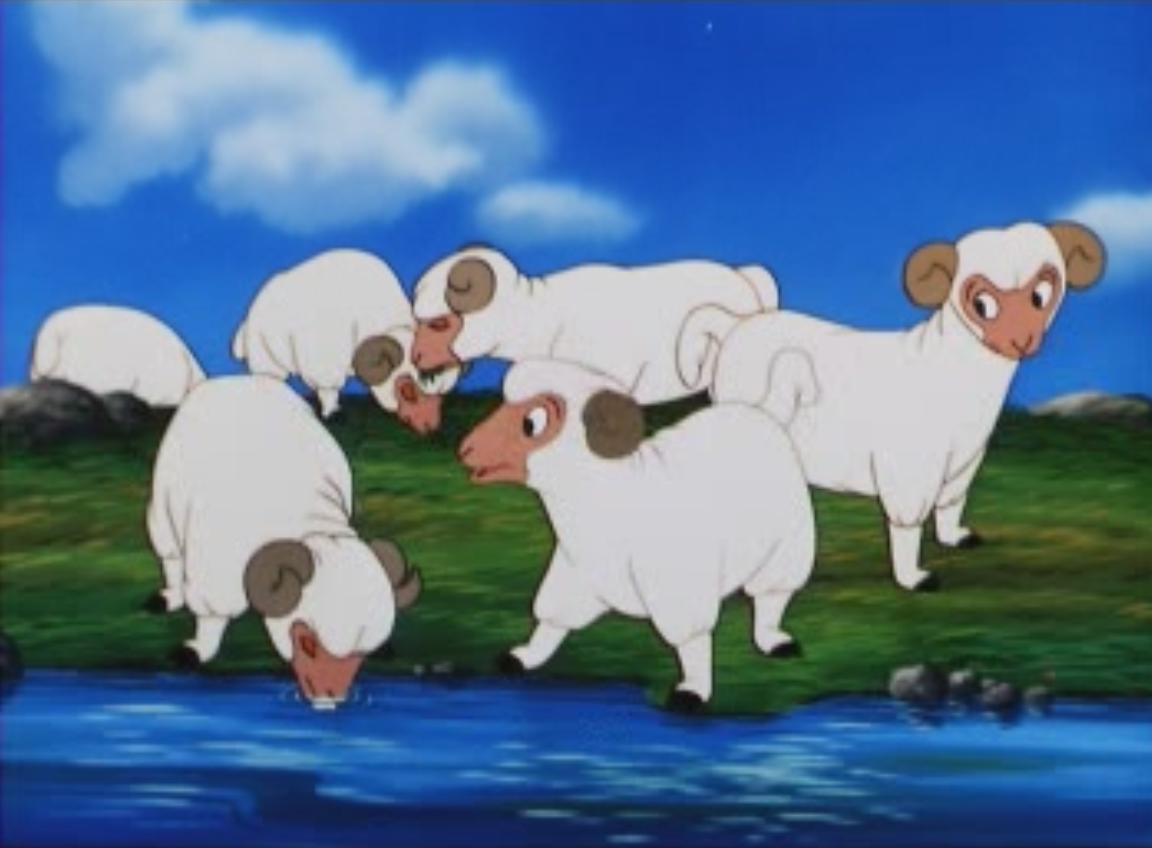
\includegraphics[width=0.45\textwidth]{img/sheep.jpg}

\includegraphics[width=0.45\textwidth]{img/wolf.jpg}\\
\tiny{Lambert the Sheepish Lion, dir. by Jack Hannah © Disney , 1952}
\end{frame}






\begin{frame}{Types de motifs}


\centering
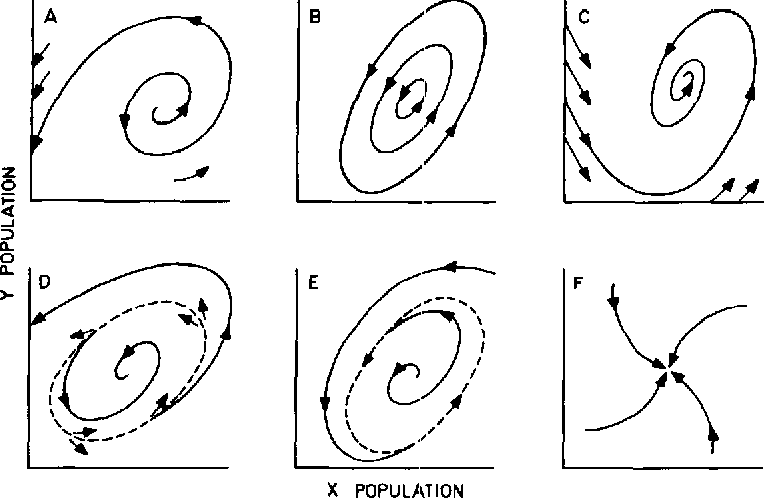
\includegraphics[width=0.5\textwidth]{img/behavior_patterns.png}\\
\flushleft



\scriptsize{A: équilibre instable, \\ B: cycles stables neutres ,\\ C: équilibre stable,\\ D: \alert{domaine d'attraction},\\ E: \alert{cycle limite stable},\\ F: point stable }

\tiny{Obtenues par résolution du système d'équation , et analyse de la matrice Jacobienne aux points fixes}


  
\end{frame}


\begin{frame}{Caractéristiques de ce genre de modèles}

\begin{itemize}
\item tous ces modèles on un point fixe ou un cycle limite stable  (théorème de Kolmogorov)
\item un modèle est soit globalement stable (et il se maintient) ou globalement instable (et il s'éteint)  
\item La stabilité neutre est très improbable ($\approx$ quand rien ne prend le dessus dans la trajectoire du système ) 
\item Quand le système est  stable, un cycle limite est probable 
\end{itemize}

\end{frame}




\begin{frame}{Complexifier les modèles}



\begin{footnotesize}

 \begin{columns}
          \column{0.48\textwidth}
             On relâche les hypothèses simplificatrices

\vspace{0.2cm}
\begin{itemize}
  \item plusieurs espèces 
\item  délai dans la reproduction (gestation) 
\item  satiété/saturation des prédateurs 
\item  prédation non-aléatoire
\item  seuil de densité d'individus pour qu'il y ait reproduction
\end{itemize}

           \column{0.55\linewidth}

$\implies$ D-type patterns \\
\vspace{1cm}
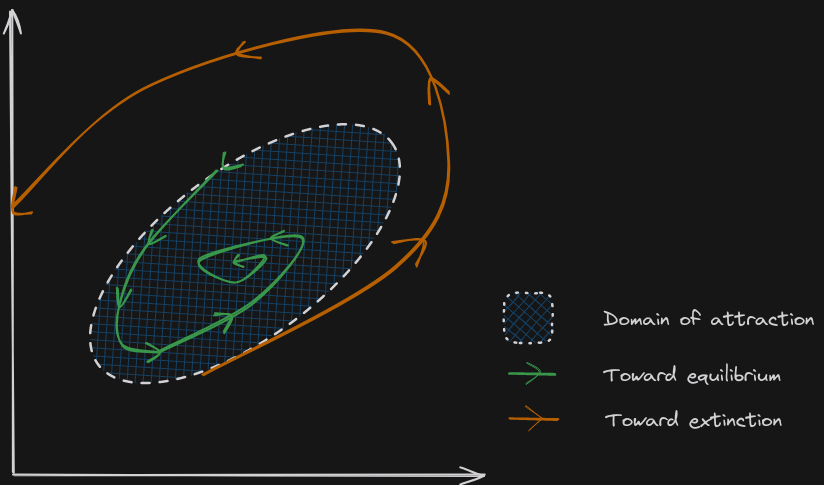
\includegraphics[width=\textwidth]{img/type2D.png}
\vfill
\end{columns}

\end{footnotesize}

\end{frame}



\begin{frame}{Domains d'attraction}


Les modèles plus réalistes ont : 



\begin{itemize}
  \item  \alert{plusieurs} domaines d'attraction 
  \item points stables,
  \item cycles limites stables 
\end{itemize}


\vfill



la \alert{taille} et  \alert{l'endroit} des domaines  $\leftrightarrow$ \alert{persistance} du système et la  \alert{probabilité d'extinction} des espèces\\


\vfill



  
\end{frame}




\begin{frame}{Netlogo demo}
\vfill
Lapins, trèfle et herbe en Netlogo
\vfill
\centering

\includegraphics[width=0.6\textwidth]{img/bunny.jpg}

\tiny{Big Buck Bunny, The Blender Fondation, 2008}

  
\end{frame}

\begin{frame}{Quelles différences avec les équations ? }

Netlogo ajoute : 

\begin{itemize}
  \item des populations discrètes (i.e. pas continues, $\in \mathbb{N}$) 
  \item trois "espèces"
  \item aléatoires
  \item de l'espace et du mouvement
\end{itemize}


\end{frame}




\section{Systèmes naturels réels}



\begin{frame}{Un lac}
\begin{footnotesize}
 \begin{columns}
           \column{0.48\textwidth}
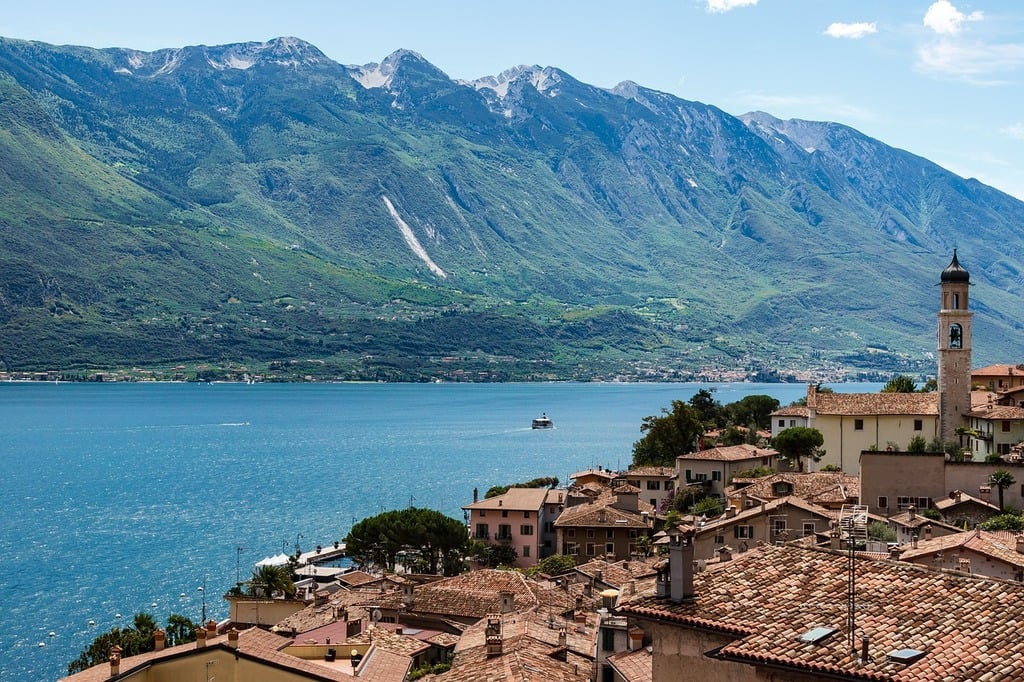
\includegraphics[width=\textwidth]{img/lake_garda_italy.jpg}
\tiny{Garda Lake, Italy (CC)}
          \column{0.58\textwidth}
          
Bonnes propriétés : 
\begin{itemize}
  \item  presque fermé (bassin versant)
  \item  les poissons sont mobiles à l'intérieur
  \item  une masse d'eau suffisante pour encaisser les variations climatiques 
  \item  beaucoup de perturbations humaines sont documentées 
\end{itemize}

Deux types de perturbations (appelé \alert{contrôles}, cf. thermostat): 

\begin{itemize}
\item nutriments des poissons :  déchets humains ou industriels déversés 
\item la pêche   
\end{itemize}
\end{columns}
\end{footnotesize}
\vfill
Comment ces interactions réelles modifient les motifs théoriques ?  (ceux issus des équations)  
 
\end{frame}

\begin{frame}{Il était une fois un lac }



Les \alert{paleolimnologistes} sont les archéologistes/plaléontologistes des lacs. Ils analysent les sédiments pour décrire comment les lacs ont évolué.

\vfill

Un lac en Italie : 


\begin{footnotesize}
\begin{enumerate}
\item pendant des milliers d'années \alert{équilibre} entre les espèces $\approx$ rien ne bouge  (2000 av. J.-C. to 171 av. J.-C.), même si les alentours changent (steppes $\rightarrow$ prairies $\rightarrow$ forêts)
\item  \alert{Changement soudain} dû à une perturbation externe : une voie romaine arrive au bord du lac (Via Cassia) en 171 av. J.-C. 
\item la population humaine augmente, \alert{pêche} et mets ses \alert{déchets dans le lac}.
\item \alert{Eutrophication} : l'environnement devient riche en éléments N et  P ($\implies$ changement subtils dans les régimes hydrographiques :  algues , plancton)  
\item Nouvelles dynamiques des populations animales, \alert{changements radicaux et irréversibles}
\end{enumerate}
\end{footnotesize}
\end{frame}





\begin{frame}{D'autres lacs}

\begin{footnotesize}
On retrouve  le même motif dans d'autres lacs (Italie, Canada, US) , avec d'autres espèces de poissons  (esturgeons, harengs, carpes  ) 

\begin{itemize}
  \item pêche intensive pendant longtemps
  \item puis  \alert{chute soudaine} des populations de poissons (quatre ordres de grandeur en quelques années)
  \item apparition ou disparitions d'espèces (insectes, plancton, vers, poissons )
  \item larges oscillations
  \item le système se positionne dans un nouveau \alert{domaine d'attraction}
\end{itemize}
\end{footnotesize}
\centering
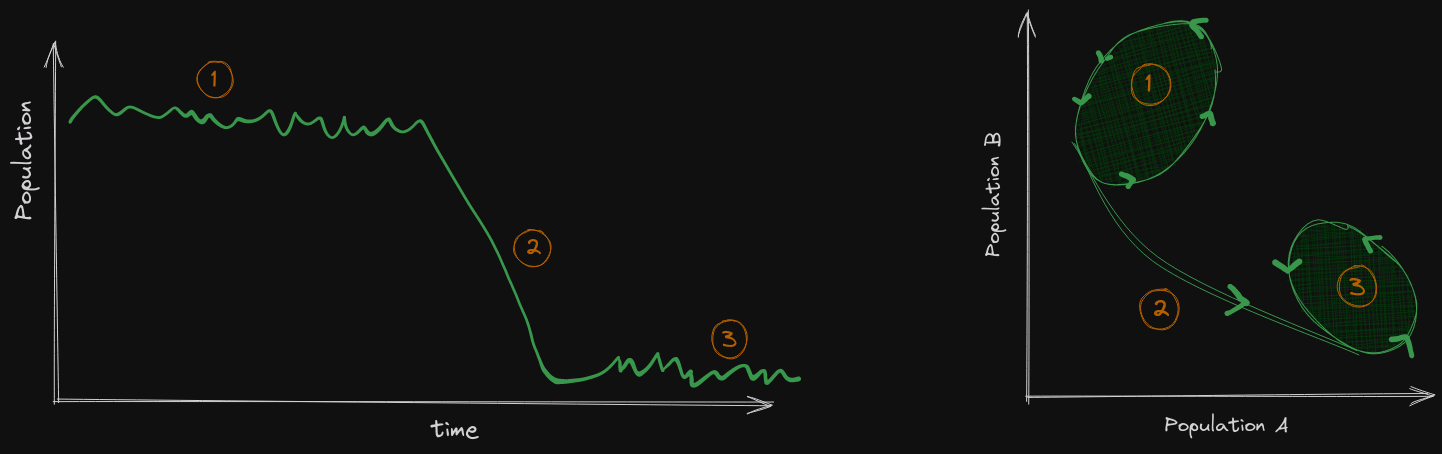
\includegraphics[height=0.4\textheight]{img/pattern_in_lake.png}


\end{frame}


\begin{frame}{Explications biologiques}


\textit{"It is as is the population had been shifted by fishing pressure from a domain with a high equilibrium to one with a lower one"}

\vfill

\begin{footnotesize}
\begin{itemize}
  \item La pêche altère la pyramide des âges des poissons : beaucoup de juvéniles, peu d'adultes, moins de reproductions
  \item Forte pression de la pêche + modification de la chimie de l'environnement  $\implies$ apparition de nouveaux compétiteurs, proies et prédateurs 
  \item Si on exploite au rendement maximum des poissons , une petite surmortalité suffit à \alert{effondrer le système}
\end{itemize}


\end{footnotesize}




\end{frame}

\begin{frame}{Premières Conclusions}

\begin{itemize}
\item C'est la pêche intensive qui a progressivement réduit la  \alert{résilience} des poissons
\item La capacité d'absorption des lacs est importante , mais pas infinie
\item Quand la limite est franchie, le système  rejoint un autre domaine d'attraction
\item La plupart des systèmes ont plusieurs domaines d'attractions
\end{itemize}

\end{frame}


\begin{frame}{Vocabulaire}


\begin{block}{\alert{Resilience}}  "a measure of the \alert{persistence} of systems and of their \alert{ability to absorb change} and disturbance and still \alert{maintain
the same relationships} between populations or state variables"
\end{block}

\vfill
\begin{block}{\alert{Résilience}}  "une mesure de la capacité d'un système à \alert{persister}, en particulier par l'\alert{absorption} des perturbations et par la capacité à  \alert{maintenir les mêmes relations} entre perturbations et variables d'état "
\end{block}


\vfill


\tiny{La définition varie selon les disciplines}\\
\tiny{Variable d'état : tout ce qui se mesure pour qualifier un système e.g. la température, la concentration en algue d'une eau, la population d'une espèce, la position et la vélocité d'un solide, etc.}



\end{frame}





\begin{frame}{Extensions}



\begin{small}
\begin{itemize}
  \item Fécondité, mortalité , compétition et prédation : \alert{Courbes de reproduction }
  \item  L'environnement n'est plus fermé, ni aléatoire, ni homogène : \alert{Hétérogénéité spatiale} 
  \end{itemize}


\end{small}
  
\end{frame}




\section{Courbes de reproduction }



\begin{frame}{Courbes de reproduction}
\begin{small}
La densité des animaux se "régule" elle-même : 

\begin{itemize}
  \item faible densité : difficulté à trouver des partenaires : densité $\searrow$
  \item haute  densité : compétition pour les partenaire, la nourriture, les sites de nidification  :  densité $\searrow$
\end{itemize}

(cela modifie aussi la densité des espèces voisines dans le réseau trophique)
\end{small}
\vfill 

Les courbes de reproduction modélisent cette régulation.


\end{frame}


\begin{frame}{Courbes de Reproduction}


\centering
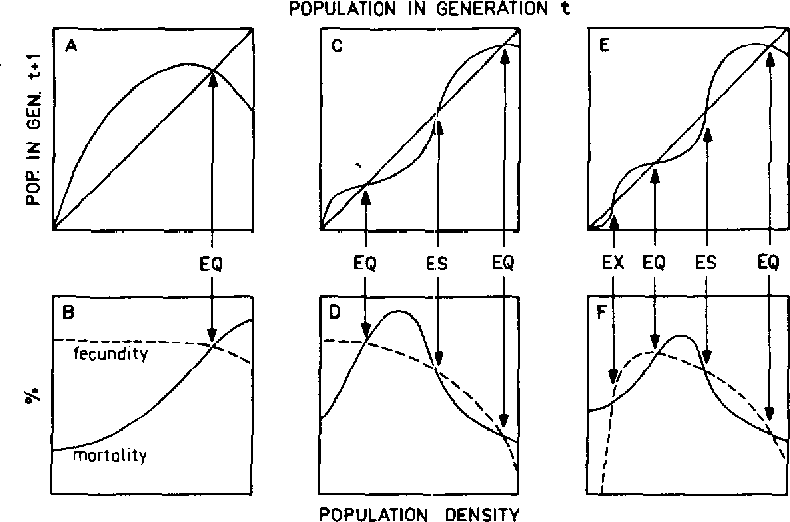
\includegraphics[height=0.5\textheight]{img/reproduction_curves.png}
\begin{footnotesize}
\begin{itemize}
\item EQ est un  \alert{équilibre}
\item ES est un  \alert{seuil d'échappement} ($\approx$ point de bascule)
\item EX est un  \alert{seuil d'extinction }
\end{itemize}

  \end{footnotesize}

\end{frame}


\begin{frame}{Courbes de Reproduction}

\vfill
\centering
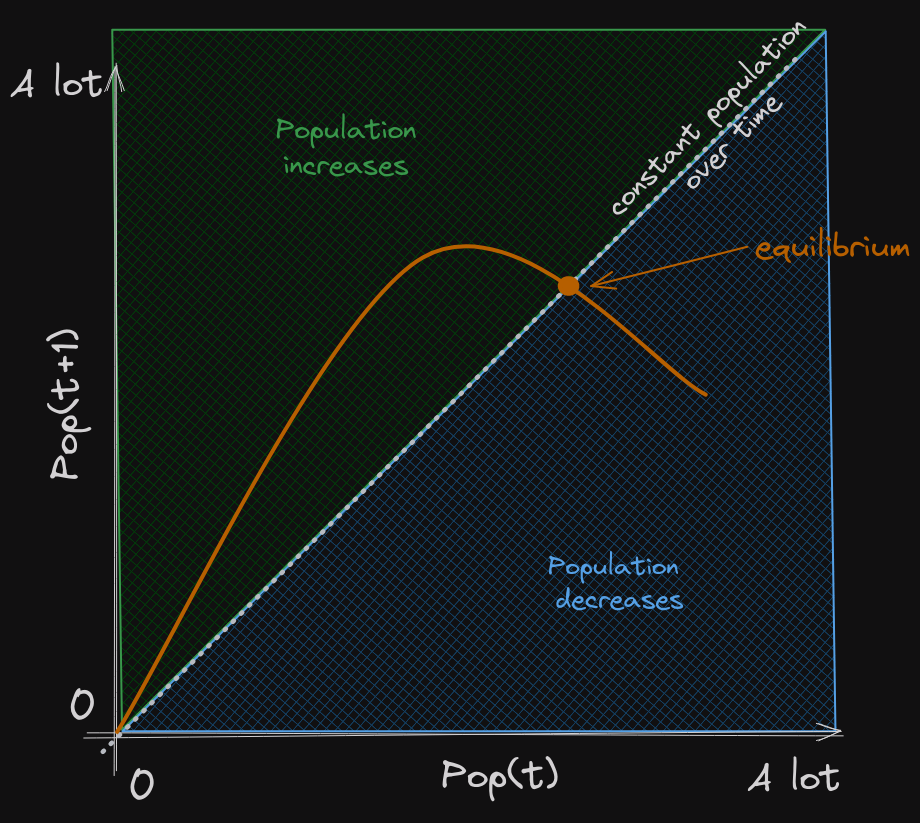
\includegraphics[height=0.8\textheight]{img/repro1.png}
\begin{footnotesize}
\end{footnotesize}

\end{frame}



\begin{frame}{Contributions de la fécondité et de la mortalité}

\vfill
\centering
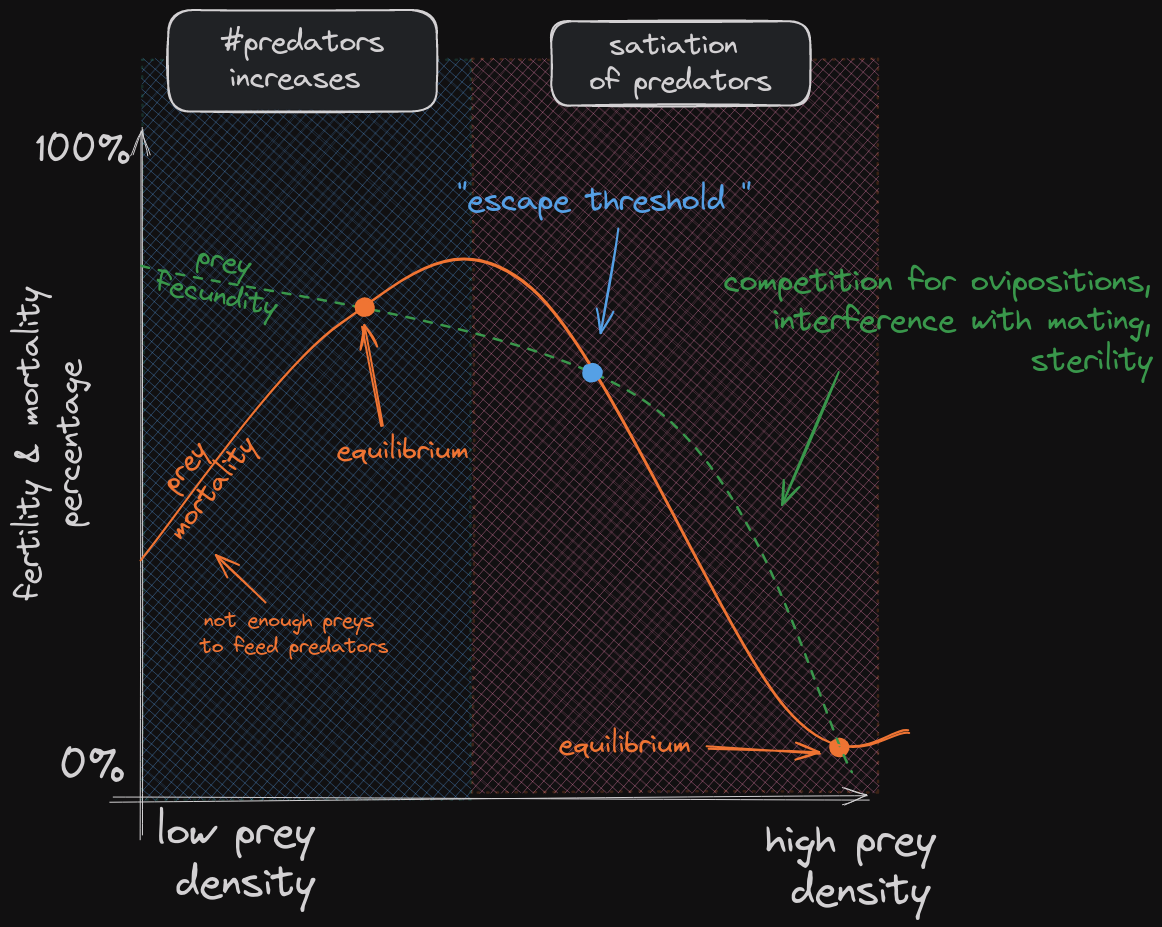
\includegraphics[height=0.8\textheight]{img/repro2.png}
\begin{footnotesize}
\end{footnotesize}

\end{frame}




\begin{frame}{Courbes de Reproduction}


\centering
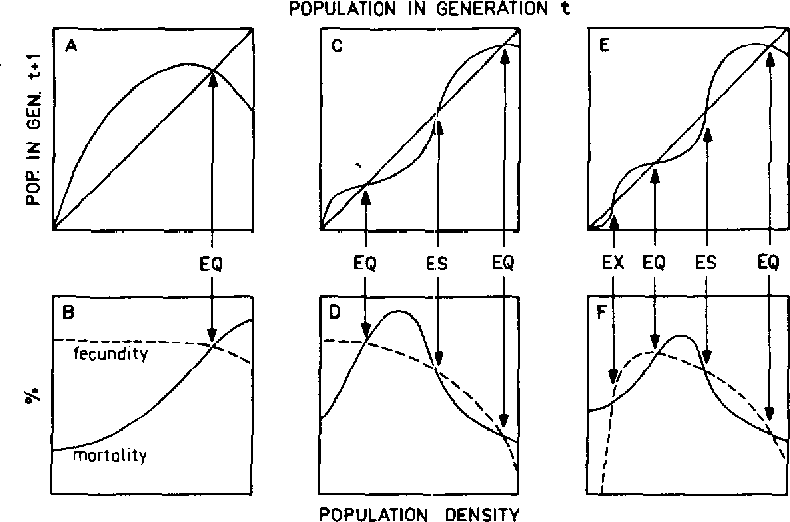
\includegraphics[height=0.5\textheight]{img/reproduction_curves.png}
\begin{footnotesize}
\begin{itemize}
\item B n'est pas réaliste , il n'inclut que les conséquences de la surpopulation
\item D est appelé  courbe \alert{Drosophile -type} 
\item F a été démontré empiriquement pour les  \alert{insectes}
\end{itemize}

  \end{footnotesize}

\end{frame}



\begin{frame}{Conclusions}


\centering
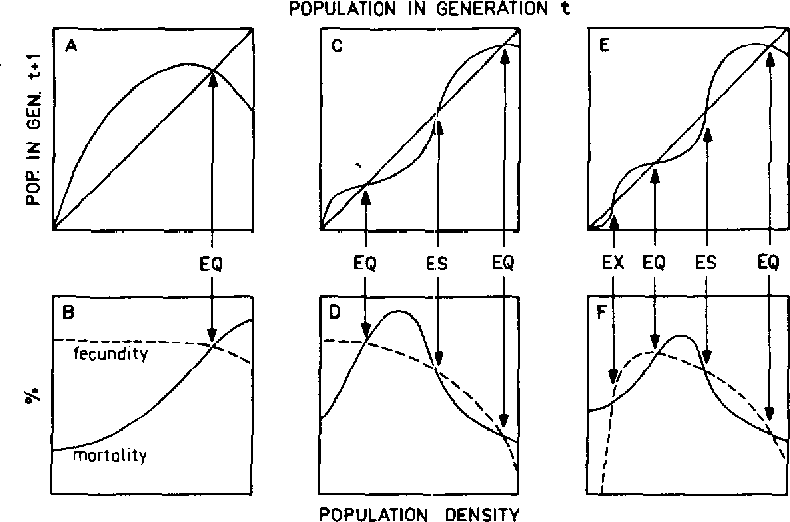
\includegraphics[height=0.5\textheight]{img/reproduction_curves.png}
\begin{footnotesize}
\begin{itemize}
\item C/D \& E/F à l’œuvre dans la nature   
\item des seuils de densité  \alert{en dessous duquel} les proies s'éteignent 
\item des seuils de densité  \alert{au dessus duquel} les proies s'éteignent 
\item Il y a des domaines d'attraction, mais pas de stabilité globale 
\item Des courbes plus complexes sont possibles 
\end{itemize}

  \end{footnotesize}

\end{frame}






\section{Systèmes réels ouverts}



\begin{frame}{Prairie, forêts et chenille}


Étude longitudinale d'une forêt de conifères et bouleaux au Canada \\
\vfill
Infestation de \alert{tordeuses}, chenille parasite des conifères.\\
\vfill
Après plusieurs années de sécheresse, des invasion de tordeuses font disparaitre les sapins (7 disparitions depuis 1700)
\vfill



\centering 
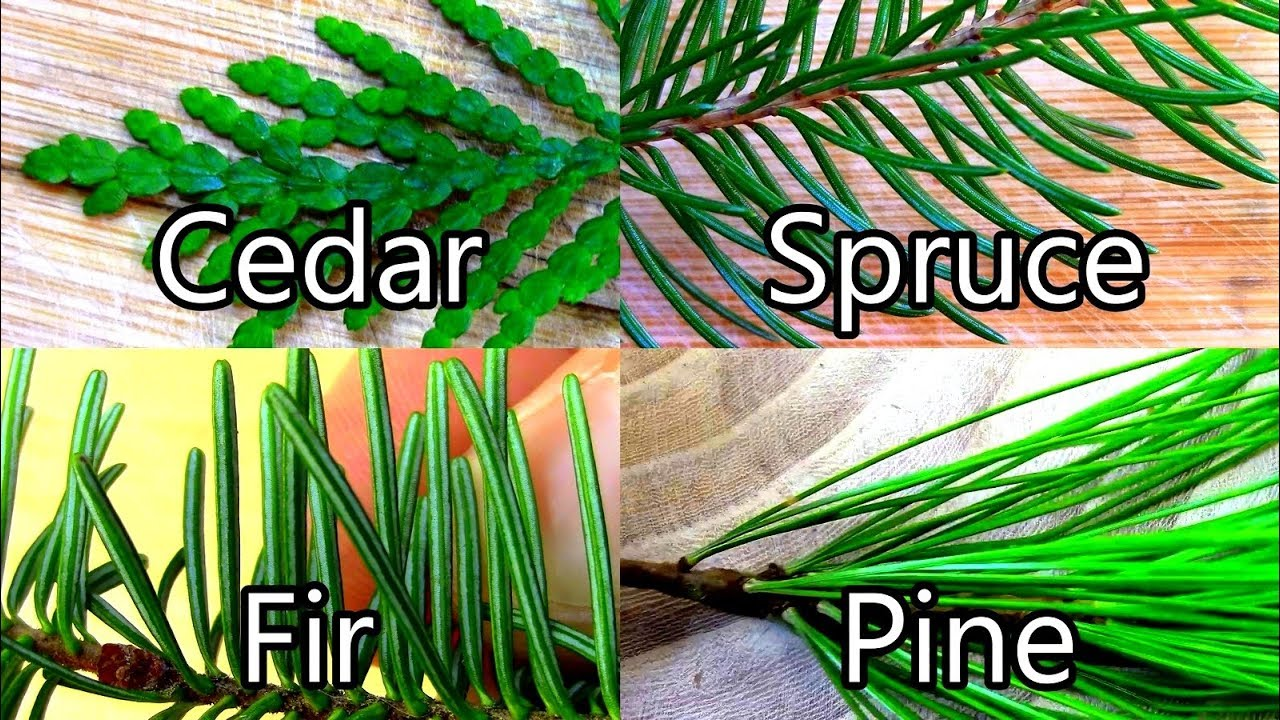
\includegraphics[height=0.3\textheight]{img/fir_spruce_pine_cedar.jpg}
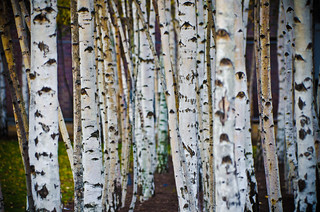
\includegraphics[height=0.3\textheight]{img/birch.jpg}
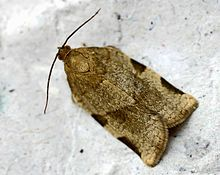
\includegraphics[height=0.3\textheight]{img/spruce_budworm.jpg}\\
\tiny{Choristoneura est un papillon de la famille des Tortricidae. PLusieurs espèces sont des ravageurs de conifères}

\vfill

\end{frame}


\begin{frame}{Deux régimes}


\begin{small}
\begin{columns}
\column{0.5\textwidth}
  \begin{block}{\alert{Pendant l'invasion}} 
  la population de chenilles explose ( $\times 10^4$) \\
  Les sapins disparaissent\\ 
  les pins et les bouleaux survivent (plus résistants à la tordeuse)
  \end{block}
\column{0.5\textwidth}
  \begin{block}{\alert{Entre les invasions}}
  Chenilles régulées par des parasites et des prédateur\\
  Régénérations des sapins  $\rightarrow$ densification des forêts\\
  les pins et les bouleaux souffrent de surpopulation , les sapins dominent  
  
  \end{block}
\end{columns}
\end{small}

\vfill

Du point de vue des arbres   :\\
 \alert{cycle limite stable}  : oscillations de large amplitude

Du point de vue des chenilles : \\
  système très instable (population varie grnadement )\\
 \alert{2 bassins d'attraction distincts}: un pour les populations normales , un pour les invasion de chenille 




\end{frame}
\begin{frame}{Survie des espèces}


\begin{itemize} 
\item Les bouleaux et pins seraient exclus de la forêt par les sapins si il n'y avait pas d'invasion
\item Les sapins survivent car ils peuvent repousser et grâce à l'effet conjugué de des croissances des autres arbres et des conditions climatiques favorables à l'invasion de chenilles
\item Ces fluctuations essentielles pour le maintien des chenilles  : les générations successives d'arbres assurent un renouvèlement de nourriture pour les futures générations , ainsi que leur prédateurs et leurs proies (les arbres). le système  $\{chenilles, predateurs, arbres\}$ se maintient aussi
\end{itemize}
\vfill
le système $\{chenille, foret\}$ est très \alert{instable} et pourtant très \alert{résilient}
\vfill
Motifs similaires avec les systèmes  $\{saumons,ours,fleuve\}$ prairies $\{prairies, arbres, feux \}$ 

\end{frame}





\section{Éléments d'écologie à retenir }


\begin{frame}{Résumé}



\alert{Stabilité} : capacité" à retourner à un équilibre après une perturbation\\
Caractéristiques  : degré de fluctuation  autour des états d'équilibre, le temps de retour à l'équilibre

\vfill

\alert{Résilience} : persistance des relations dans le systèmes capacités à absorber les perturbations (modification des variables d'état ou des contrôles) et à persister malgré elles \\
 La résilience se traduit par la persistance d'une espèce (ou plusieurs) ou un faible probabilité de leur extinction.


\end{frame}



\begin{frame}{Le super bol}



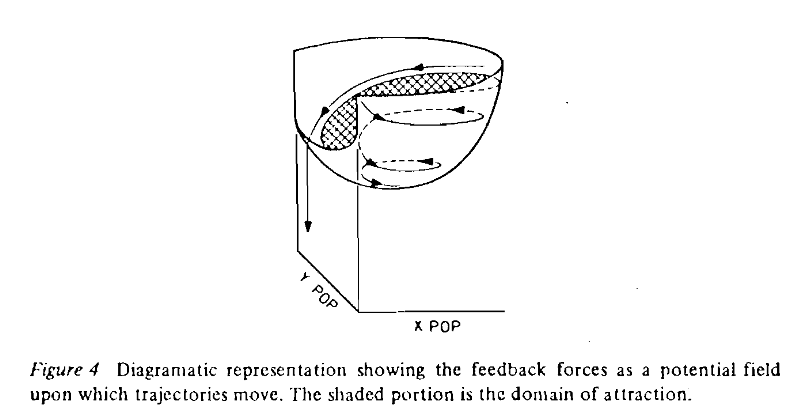
\includegraphics[height=0.8\textheight]{img/bowl.png}

\end{frame}




\begin{frame}{Résilience}
\vfill
On peut être résilient \alert{et} instable ( cf. tordeuses)
\vfill

On peut être stable mais pas résilient :  population a traversé des milliers d'années dans des conditions climatiques à peu près constantes , perd sa faculté d'adaptation aux perturbations (cf . les poissons du lac) 

\vfill
Quand les systèmes sont \alert{ouverts}, et les espèces capables de \alert{se disperser}, ils sont résilients (e.g. sauterelles, méduses )

\vfill

\end{frame}
\begin{frame}{Systèmes complexes vulgarisés}


 La diversité est liée à la stabilité . \\

 Stabilité est, en gros, le nombre de flèches dans un réseau trophique  

\vfill

 
 plus un système est complexe, plus il fluctue

\vfill

 + d'espèces $\implies$ + de  domaines d'attraction. \\

 Malgré des fluctuations plus importantes, le système peut persister. 
 



\end{frame}


\section{les derniers mots}

\begin{frame}{À retenir}

\begin{itemize}
 \item la Nature, c'est dur (à modéliser)
 \item Tout a un effet sur tout, tout le temps 
 \item Impossible de tout mesurer, ou quantifier 
 \item Les outils mathématiques traditionnels sont rarement utiles ( la simulation peut aider )
 \item Le point de vue des équilibres est rarement utile, ou vrai  
 \item Plusieurs bassins d'attraction et cycles limites, le système "navigue" parmi eux 
\end{itemize}

\end{frame}


\begin{frame}{Resilience dans d'autres disciplines}

\begin{small}
\alert{Resilience en ingénieurie} : la capacité d'un système à retrouver sa position d'équilibre après une perturbation \alert{temporaire}, en mesurant à quelle vitesse l'équilibre est retauré (Pimm 1984, Holling 1996).\\
Définition incomplète selon moi : c'est le retour au même point qui est mesuré ici, pas le maintien des relations entre les éléments. Une voiture crevée reoule encore !

\vfill

\alert{la résilience socio-technique }  i.e. les points communs trouvés dans beaucoup de définitions : 
\begin{itemize}
  \item  \alert{Adaptabilité} et flexibilité 
  \item  La capacité à s'auto-organiser 
  \item  La capacité à  \alert{apprendre et s'adapter} (et favoriser les conditions )
  \item  La capacité à maintenir des \alert{liens}  avec d'autres systèmes 
  \end{itemize}
\end{small}


\end{frame}



\begin{frame}{Mon point de vue}

\begin{itemize}
\item  Holling a un point de vue original et iconoclaste : \alert{\textit{Il n'y a (presque) pas d'équilibre et d'harmonie dans la nature}}
\item un des meilleurs papiers que j'aie jamais lus 
\item impact majeur dans l'écologie 
\item des concepts faciles à apprendre , difficile à maîtriser 
\item le terme de résilience est repris partout (souvent n'importe comment)
\item Holling propose un \textit{paradigme} : une façon de voir les choses qui peut être appliquée partout 
\end{itemize}


\end{frame}


\begin{frame}{plus jamais de confusion entre robustesse et résilience }

\centering
 Qui est le plus résilient ? 


\includegraphics[height=0.8\textheight]{img/wolverine_colossus.jpg}

\tiny{Cover by Mark Bagley,  © Marvel }

\end{frame}







\begin{frame}{References}


The paper : \url{https://pure.iiasa.ac.at/id/eprint/26/1/RP-73-003.pdf}

Ecosystem models wikipedia page (a good introduction) : \url{https://en.wikipedia.org/wiki/Ecosystem_model} \\

Holling's carreer overview \url{ https://www.nature.com/articles/s41893-019-0425-9\#ref-CR4}

Netlogo Cinematic Universe : \url{https://ccl.northwestern.edu/netlogo/}


\end{frame}




\begin{frame}[standout]

\centering
Thank You\\
\vfill
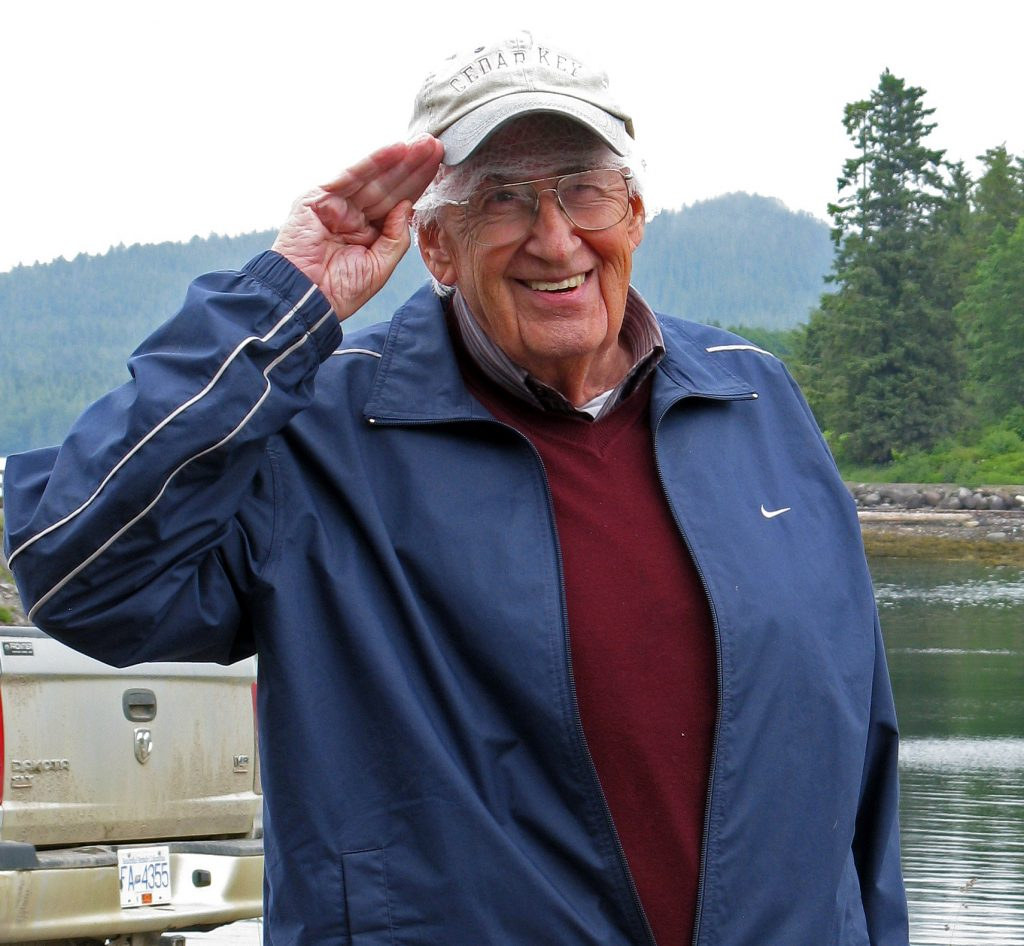
\includegraphics[height=0.9\textheight]{img/holling2.jpg} \\
\tiny{photo from Ecotrust Canada website}
  
\end{frame}






\begin{comment}


\section{Predator and prey}



@article{Pethybridge2018ImprovingME,
  title={Improving Marine Ecosystem Models with Biochemical Tracers.},
  author={Heidi R. Pethybridge and C. Anela Choy and Jeffrey Joseph Polovina and Elizabeth A. Fulton},
  journal={Annual review of marine science},
  year={2018},
  volume={10},
  pages={
          199-228
        },
  url={https://api.semanticscholar.org/CorpusID:207741887}
}
\end{comment}

\end{document}
